%%%%%%%%%%%%%%%%%%%%%%%%%%%%%%%%%%%%%%%%%%%%%%%%%%%%%%%%%%%%%%%%%%%%%%%%%%%%%%%%
%2345678901234567890123456789012345678901234567890123456789012345678901234567890
%        1         2         3         4         5         6         7         8

\documentclass[letterpaper, 10 pt, mydraft, conference]{ieeeconf}  % Comment this line out if you need a4paper

%\documentclass[a4paper, 10pt, conference]{ieeeconf}      % Use this line for a4 paper

\IEEEoverridecommandlockouts                              % This command is only needed if 
                                                          % you want to use the \thanks command

\overrideIEEEmargins                                      % Needed to meet printer requirements.

% See the \addtolength command later in the file to balance the column lengths
% on the last page of the document

% The following packages can be found on http:\\www.ctan.org
%\usepackage{graphics} % for pdf, bitmapped graphics files
%\usepackage{epsfig} % for postscript graphics files
%\usepackage{mathptmx} % assumes new font selection scheme installed
%\usepackage{times} % assumes new font selection scheme installed
%\usepackage{amsmath} % assumes amsmath package installed
%\usepackage{amssymb}  % assumes amsmath package installed

\usepackage[english]{babel}

\usepackage{graphics} 		% for pdf, bitmapped graphics files
\usepackage{graphicx}
\usepackage{epsfig} 		% for postscript graphics files
\usepackage{epstopdf}

\usepackage{listings}
\usepackage{color}
\usepackage{nameref}
\usepackage[bookmarks=true]{hyperref}
\usepackage[colorinlistoftodos]{todonotes}
%\usepackage{index}
%\usepackage{pgfgantt}
\usepackage{amsmath}	 	% assumes amsmath package installed
\usepackage{amssymb}  		% assumes amsmath package installed

\usepackage{dsfont}
\usepackage{mathtools}

\usepackage{epigraph}
\usepackage{lscape}
\usepackage[]{nomencl}		% nomenclatures
\usepackage[ruled,vlined]{algorithm2e}
\usepackage{multicol}
\usepackage{multirow}
\usepackage{etoolbox}

\usepackage{caption}
\usepackage[labelformat=simple]{subcaption}
\renewcommand\thesubfigure{(\alph{subfigure})}
\usepackage{wrapfig}

%\usepackage{flushend}

\usepackage{units}
%\usepackage{flushend}


\pdfminorversion=4

%========================================================
% GENERAL
%--------------------------------------------------------

\renewcommand{\sec}{Section~}
\newcommand{\fig}{Fig.~}
\newcommand{\eq}{}
\newcommand{\app}{Appendix~}
\newcommand{\tab}{Table~}
\newcommand{\alg}{Alg.~}
%\newcommand{\line}{Line~}

\newcommand{\newword}[1]{\textbf{#1}}

%\newindex{todo}{tod}{tnd}{TODO List} % start todo list
%\newindex{fixme}{fix}{fnd}{FIXME List} % start fixme list
%\newcommand{\todo}[1]{\textcolor{blue}{TODO: #1}\index[todo]{#1}} % macro for todo entries
%\newcommand{\fixme}[1]{#1}
%\DeclareOption{mydraft}{\renewcommand{\fixme}[1]{\textcolor{red}{\textbf{#1}}}}
%\ProcessOptions

\newcommand{\fixme}[1]{}
\DeclareOption{mydraft}{\renewcommand{\fixme}[1]{\textcolor{red}{#1}}} 		% macro for fixme entries
\ProcessOptions
\newcommand{\comment}[1]{}
\DeclareOption{mydraft}{\renewcommand{\comment}[1]{\textcolor{blue}{\textbf{[NdR: #1]}}}}		% macro for comment
\ProcessOptions

% Colors used in Matlab plots
\definecolor{matlab1}{rgb}{0,0,1}
\definecolor{matlab2}{rgb}{0,0.5,0}
\definecolor{matlab3}{rgb}{1,0,0}
\definecolor{matlab4}{rgb}{0,0.75,0.75}
\definecolor{matlab5}{rgb}{0.75,0,0.75}
\definecolor{matlab6}{rgb}{0.75,0.75,0}
\definecolor{matlab7}{rgb}{0.25,0.25,0.25}


\definecolor{darkgreen}{rgb}{0,0.5,0}		%Olivegreen?
\definecolor{purple}{rgb}{0.75,0,0.75}
\definecolor{pink}{rgb}{1,0.4,0.6}


\newcommand{\specialcell}[2][c]{%
  \begin{tabular}[#1]{@{}c@{}}#2\end{tabular}}
  
\newcommand{\unknown}[0]{\fixme{XXX}}
\newcommand{\missingcitation}[0]{\fixme{\cite{???}}}

\providecommand{\SetAlgoLined}{\SetLine}
\providecommand{\DontPrintSemicolon}{\dontprintsemicolon}


%========================================================
% MATH
%--------------------------------------------------------

\renewcommand{\vec}{\boldsymbol}				% Vector
\newcommand{\mat}{\boldsymbol}					% Matrix
\DeclareMathOperator{\diag}{\mathrm{diag}} 			% Diagonal matrix

\newcommand{\R}[0]{\mathds{R}}					% Real numbers

\renewcommand{\d}{\mathrm{d}}					% Derivate
\newcommand{\gradient}{\nabla}					% Gradient
\newcommand{\hessian}{H}					% Hessian
\nomenclature{\hessian}{Hessian}

\newcommand{\inv}[0]{^{-1}} 					% Inverse
%\newcommand{\T}[0]{^T} 						% Transpose % \top
\newcommand{\T}[0]{^\top} 						% Transpose % \top

\newcommand{\norm}[1]{\left|\left| #1 \right|\right|} 		% Norm
\newcommand{\asin}[0]{\sin^{-1}} 	% 

\newcommand{\E}{\mathds{E}}	 				% expectation operator
\DeclareMathOperator{\var}{\mathrm{var}} 			% variance
\newcommand{\prob}{{p}} 					% probability density function
\newcommand{\normcdf}[1]{\Phi\left( #1 \right)} 		% Normal Cumulative distribution function
\newcommand{\normpdf}[1]{\phi\left( #1 \right)} 		% Normal probability density function
\newcommand{\gauss}[2]{\mathcal{N} \left( #1,#2 \right)}	% Gaussian Distribution


%========================================================
% MACHINE LEARNING
%--------------------------------------------------------

\newcommand{\dataset}[0]{\mathds{D}} 				% Dataset
\newcommand{\trainingset}[0]{\mathcal{D}}

\newcommand{\inputMatrix}[0]{\mat x}
\newcommand{\inputSpace}[0]{\mathcal{X}}
\newcommand{\outputMatrix}[0]{\mat y}
\newcommand{\regressionNo}[0]{f}

%========================================================
% GAUSSIAN PROCESSES
%--------------------------------------------------------

%\newcommand{\GP}[0]{\text{GP}} % Gaussian process
\newcommand{\GP}[0]{\mathcal{GP}} 	% Gaussian Process
\newcommand{\noise}[0]{w}

%========================================================
% OPTIMIZATION
%--------------------------------------------------------

\DeclareMathOperator*{\argmin}{arg\,min}
\DeclareMathOperator*{\minimize}{\text{minimize}}
\newcommand{\parameters}[0]{\vec x} 			% Parameters
\newcommand{\dimparameters}{d}					% Dimensionality parameters
\newcommand{\iteration}[0]{i}

\newcommand{\objfuncNo}[0]{f}					% Objective function
\newcommand{\objfunc}[1]{\objfuncNo\left(#1\right)}		% Objective function (as a function)
\newcommand{\respsurfNo}[0]{\hat \objfuncNo}			% Response surface
\newcommand{\respsurf}[1]{\respsurfNo \left( #1 \right)} 	% Response surface (as a function)
\newcommand{\acqfuncNo}[0]{\alpha}				% Acquisition function
\newcommand{\acqfunc}[1]{\acqfuncNo \left( #1 \right)}		% Acquisition function (as a function)
\newcommand{\acqsurf}[1]{\acqfuncNo \left( #1 \right)}		% Acquisition surface
\newcommand{\gradientline}{\d \objfunc{\parameters}/\d \parameters}

% Multi-objective optimization
\newcommand{\numbersubobj}[0]{n}
\newcommand{\mergefuncmooNo}[0]{z}
\newcommand{\mergefuncmoo}[1]{\mergefuncmooNo \left( #1 \right)}
\newcommand{\weightsmoo}[0]{\alpha}
\newcommand{\subobjfuncNo}[0]{g}
\newcommand{\subobjfunc}[1]{\subobjfuncNo \left( #1 \right)}


%========================================================
% Neural Networks
%--------------------------------------------------------

\newcommand{\nntf}[1]{\sigma \left( #1 \right)} 		% Neural Networks Transfer function
\newcommand{\nnBh}[0]{\vec {Bh}} 				% Neural Networks Bias of Hidden layer
\newcommand{\nnB}[0]{\vec B} 					% Neural Networks Bias
\newcommand{\nnW}[0]{\mat W} 					% Neural Networks Weights
\newcommand{\nnE}[0]{E} 					% Neural Networks Error function


%========================================================
% ROBOTICS
%--------------------------------------------------------

\newcommand{\q}{\mat q}
\newcommand{\dq}{\dot{\q}}
\newcommand{\ddq}{\ddot{\q}}
\newcommand{\skinInput}{\mathcal{\vec S}}

\newcommand{\frictionMatrixNo}[0]{\mat f}
\newcommand{\inertiaMatrixNo}[0]{\mat M}
\newcommand{\inertiaMatrix}[0]{\inertiaMatrixNo \left( \q \right)}
\newcommand{\gravityMatrixNo}[0]{\vec g}
\newcommand{\torque}{\tau}
\newcommand{\torques}[0]{\vec \torque}
%\newcommand{\forceNo}[0]{\vec F}
\newcommand{\extForce}[0]{\gamma}
\newcommand{\extForces}[0]{\vec \extForce}
\newcommand{\ftsForce}{F}
\newcommand{\ftsForces}{\vec \ftsForce}
\newcommand{\jtsForce}{\tau}%_text{JTS}}
\newcommand{\jtsForces}{\vec \jtsForce}%_text{JTS}}
\newcommand{\Hmatrix}[0]{\vec h \left(\q,\dq \right)}
\newcommand{\jacobian}[0]{\mat J}
\newcommand{\coriolis}[0]{C}

%========================================================
\ProcessOptions
%========================================================

\newcommand{\idyn}[0]{\textit{iDyn}}

\newcommand{\robot}{\textit{iCub}}

\newcommand{\figspace}{\vspace{-10pt}}


\title{\LARGE \bf
%Learning Whole-Body Control with Tactile Sensing
%Learning forward and inverse dynamics of contacts using tactile sensing
%Learning dynamics models of contacts using tactile sensing
%Predicting Joint Torques in Inverse Dynamics Models with Contacts
Learning Inverse Dynamics Models with Contacts
}


\author{Roberto Calandra$^{1}$, Serena Ivaldi$^{1,2}$, Marc Peter Deisenroth$^{3}$, Elmar Rueckert$^{1}$, Jan Peters$^{1,4}$% <-this % stops a space
\thanks{*The research leading to these results has received funding from the European Community's Seventh Framework Programme (FP7/2007--2013) under grant agreements \#270327 (CompLACS) and \#600716 (CoDyCo). MPD has been supported by an Imperial College Junior Research Fellowship.}% <-this % stops a space
\thanks{We thank V. Padois and A. Droniou for their help with \textit{iCubParis02}.}
\thanks{$^{1}$Intelligent Autonomous Systems, TU Darmstadt, Darmstadt, Germany}%
\thanks{$^{2}$Inria, Villers-l\`es-Nancy, F-54600, France; CNRS, Loria, UMR n.7503 and Universit\'e de Lorraine, , Vandoeuvre-l\`es-Nancy, F-54500, France}%
\thanks{$^{3}$Department of Computing, Imperial College London, London, UK}%
\thanks{$^{4}$Max Planck Institute for Intelligent Systems, T\"ubingen, Germany} %
}

\begin{document}



\maketitle
\thispagestyle{empty}
\pagestyle{empty}


%%%%%%%%%%%%%%%%%%%%%%%%%%%%%%%%%%%%%%%%%%%%%%%%%%%%%%%%%%%%%%%%%%%%%%%%%%%%%%%%

\begin{abstract}
	% %
% %% General problem
% Controlling a robot in the presence of contacts with the environment is an open research problem. 
% In particular, one challenge needs to be addressed: the contact torques\slash forces need to be estimated.
% %
% %% Detailed problem
% % Why no torque sensors.
% % PROBLEM!!! We also need them!!!!
% In principle, the contact forces can be directly estimated with force/torque sensors. 
% However, they are expensive and cannot be integrated in all joints. 
% Additionally, the exact position of the contact \fixme{plus other stuff} must be known precisely.
% % Why no skin
% A different approach is to use tactile sensing to identify the contact forces, in conjunction with an analytic model of the contact.
% %Another approach is to use analytic models of contacts. 
% This requires the position of the sensors on the body to be precisely known. 
% Moreover, designing a model becomes complicated with an increasing number of sensors.  
% Therefore, often only an approximate contact model is known. 
% 
% %% Our contribution
% In this paper, we investigate how contact forces can accurately be learned using raw tactile sensing. 
% For this purpose, we propose a novel approach to learning a contact force model directly from data using non-parametric regression methods. 
% 
% %% Our experiments
% As a proof of concept, we validate our approach on a humanoid robot \robot{}. 
% We first show that the learned model can accurately predict the contacts force of a single contact exclusively using tactile information.
% Our approach extends to multiple contacts, and we show that it outperforms existing contact models that make use of force\slash torque sensors in situations with multiple simultaneous contacts.
%
%
%
%
%
%In many settings, robots interact with their %environment and manipulate objects.
%% General problem
%Contacts pose key research challenges when modeling and controlling a robot that interacts with its environment.
%Contacts have non-linear effects on the system dynamics that are difficult to model accurately and may cause interaction forces that could harm a robot.
%
%Therefore, for adaptive control strategies the contact torques\slash forces need to be estimated accurately. In principle this can be done through joint-torque sensors.
In whole-body control, joint torques and external forces need to be estimated accurately. In principle, this can be done through pervasive joint-torque sensing and accurate system identification.
However, these sensors are expensive and may not be integrated in all links.
Moreover, the exact position of the contact must be known for  a precise estimation. 
If contacts occur on the whole body, tactile sensors can estimate the contact location, but this requires a kinematic spatial calibration, which is prone to errors. 
Accumulating errors may have dramatic effects on the system identification.
%
% REMOVE THIS?? ==>
% However, these sensors are expensive, may not be integrated in all links, and the exact position of the contact must be known. Already small deviations from the true contact location might have dramatic effects on the estimated dynamics. 
% Alternatively, tactile sensing may be used to estimate the contact location and the forces, as in existing analytically modeling approaches. Also in these methods the position of each sensor element (typical sensor arrays consist of 100--1000 elements) has to be precisely known.
%
% <== REMOVE THIS??
%Existing approaches model contacts analytically, where the position of each sensor element in the robot body (typical sensor arrays consist of 100--1000 elements) has to be precisely known.
%
% Alternatively, we can use tactile sensing to estimate the contact forces.
% % <== REMOVE THIS??
% Existing approaches model contacts analytically, where the position of each sensor element in the robot body (typical sensor arrays consist of 100--1000 elements) has to be precisely known.
% %% Our contribution
%
%
As an alternative to classical model-based approaches we propose a data-driven mixture-of-experts learning approach using Gaussian processes. 
This model predicts joint torques directly from raw data of tactile and force\slash torque sensors.
%In particular, a mixture-of-experts approach based on Gaussian processes is used to learn a mapping from tactile sensor inputs to observed contact forces.
%% Our experiments
%
We compare our approach to an analytical model-based approach on real world data recorded from the humanoid \robot{}.
We show that the learned model accurately predicts the joint torques resulting from contact forces, is robust to changes in the environment and outperforms existing dynamic models that use of force\slash torque sensor data.
\end{abstract}

%%%%%%%%%%%%%%%%%%%%%%%%%%%%%%%%%%%%%%%%%%%%%%%%%%%%%%%%%%%%%%%%%%%%%%%%%%%%%%%%

\section{Introduction}
\label{sec:introduction}

	

%%%==================================================================================================
%%% PROBLEM STATEMENT
%%%==================================================================================================

A fundamental problem for torque-controlled humanoid robots is to accurately model their dynamics in presence of contacts, e.g., during manipulation in clutter~\cite{Jain2013}, whole-body movements~\cite{Kajita2008} or ground contacts in locomotion~\cite{Calandra2014}.
Analytic models suffer from inaccurate dynamic parameters, unmodeled dynamics (e.g., friction, couplings, elasticities) and noisy sensor measurements.
With contacts, the problem is even more challenging, because of discontinuities and additional non-linearities, which are difficult to model or estimate.
%One particular reason for this challenge is that
%contacts cause non-linearities in the system dynamics, which
%are difficult to model analytically or estimate. 
Moreover, if contact locations are not fixed a priori or known with sufficient precision, small errors in the localization of the external force can substantially deteriorate the quality of the inverse dynamics~\cite{DelPrete2012}.
%Additionally, analytic models suffer from inaccurate dynamic parameters, unmodeled dynamics (e.g., friction, couplings, elasticities) and noisy sensor measurements.
%play in the joints => can be solved kinematically

Nevertheless, many modern control strategies like inverse dynamics control~\cite{Erez2012}, computed torque control~\cite{Siciliano2009} or model predictive control approaches~\cite{Naveau2014} rely on accurate dynamic models.
% too risky: there are techniques in NMPC that do not need this 
%(or even differentiable) dynamics models.
With inaccurate dynamics models these control strategies can produce suboptimal policies, by not taking the external forces (caused by contacts) into account, and even damages to the hardware.

%%%==================================================================================================
%%% OUR CONTRIBUTION
%%%==================================================================================================
%
\begin{wrapfigure}{r}{0.30\columnwidth}
%\begin{figure}[t]
	\vspace{-10pt}
	\centering
	\includegraphics[width=.999\linewidth]{robertoIROS/fig/iCubDarmstadt01_new}
	\caption{The humanoid robot \robot{} used in the experiments.}
    \vspace{-10pt}
	\label{fig:icub}
%\end{figure}
\end{wrapfigure}
%
%%-------------------------------------
%% Our approach
%%-------------------------------------
%
%As a first step toward a more informed controller that explicitly considers the effect of contacts, we propose to learn the dynamics model from tactile sensor readings and force-torque sensors. 
In contrast to classical techniques based on the identification of dynamics parameters~\cite{Yamane2011calibration,Ogawa2014,Traversaro2013}, we propose a fully data-driven machine learning approach based on non-parametric models, where both the rigid body dynamics as well as the effect of external forces on the robot structure are learned directly from data collected on the real robot.
The proposed model makes use of the raw sensory data and does not require a kinematic/dynamics calibration~\cite{Yamane2011calibration,Ogawa2014,Traversaro2013}: in particular, it does not need a spatially calibrated model of the skin~\cite{DelPrete2011}.
As a non-linear model for the inverse dynamics we propose to learn a ``mixtures of contacts'' based on Gaussian Processes (GP).
%Each of these GP experts models a single ``type'' of contact and can be easily learned.
%However, by using a gating network that activates and deactivates the individual GP experts, it is %possible to switch between contacts and generalize to more complex environments.
% \todo[inline, color=yellow]{I don't think this bit is necessary here...\\
% As ground-truth we use joint-torque sensor measurements,
% and  we compare to a state-of-the-art analytic modeling approach
% that assumes perfect knowledge of the contact location to model external forces.
% Our approach in contrast, uses simply the tactile information to activate the experts.}
% The Gaussian processes are trained with the robot configurations (in joint angles)
% and the force measurements of the joint-torque sensors.
%
%
%============================================================
% CHANGE ME
%

%%-------------------------------------
%% Experimental results
%%-------------------------------------
%

We evaluate our model learning approach on two different tasks using the arm of the \robot{} humanoid robot~\cite{Natale2013} (see \fig\ref{fig:icub}) and compare against a state-of-the-art analytic modeling approach.
%The learned inverse dynamics model outperforms the analytic approach and we demonstrate that the model can generalize to new environmental conditions, such as changing contact locations.
%To the best of our knowledge, this is the first demonstration of how joint torques can be learned on a humanoid robot equipped with tactile and force/torque sensors in presence of contacts.
%
% 
In the first task, the learned inverse dynamics is used to compensate for an unexpected obstruction and minimize the tracking error.
In the second task, we use the learned model on a controller designed to slide along an obstruction. 
The purpose of the sliding controller is to minimize the contact forces and therefore avoid to break the motors or the artificial tendons that actuate the joints in the case of unexpected contacts.


 

%%%%%%%%%%%%%%%%%%%%%%%%%%%%%%%%%%%%%%%%%%%%%%%%%%%%%%%%%%%%%%%%%%%%%%%%%%%%%%%%%

\section{Problem Formulation}
\label{sec:problem}

	%%--------------------------------------------
%% Inverse Dynamics
%%--------------------------------------------
%Without contacts with the environment, 
The inverse dynamics of a robot with $m$ degrees of freedom can be generally described by 
%
\begin{align}
	\torques = \underbrace{\inertiaMatrix\ddq + \Hmatrix}_{\torques_\text{RBD}} + \epsilon\,(\q,\dq,\ddq) \,,
	\label{eq:tau_nocontact}
\end{align}
%
where $\q$, $\dq$ and $\ddq$ are  the joint positions, velocities and accelerations, respectively, 
%$\inertiaMatrix \in \R^{m \times m}$ is the inertia matrix and 
$\inertiaMatrix$ is the inertia matrix and 
%
\begin{align*}
	\Hmatrix = C(\q,\dq)\dq + g(\q) + F_v \dq + F_s \,\text{sgn}(\dq) %\in \R^{m \times m}
\end{align*}
%
is the matrix combining the contributions from Coriolis and centripetal, friction (viscous and static) and gravity forces.
The term $\epsilon(\q,\dq,\ddq)$ in \eq\eqref{eq:tau_nocontact} captures the errors of the model,
such as unmodeled dynamics (e.g., elasticities and Stribeck friction), inaccuracies in the dynamic parameters (e.g., masses, inertia), vibrations, couplings, and sensor noise. 
%
With a set $\mathcal{C}=\{c_1 \ldots c_n\}$ of contacts $c_i$ between the robot and the environment, \eq\eqref{eq:tau_nocontact} becomes
%
\begin{align}
	\torques = \underbrace{\inertiaMatrix\ddq + \Hmatrix}_{\torques_\text{RBD}} + \epsilon(\q,\dq,\ddq) + \color{darkgreen}{\sum_{c_i \in\mathcal{C}} {\jacobian\T_{c_i}(\q)}\, \extForces_i} \,\color{black}{,}
	\label{eq:tau_contact}
\end{align}
%
where the last term accounts for the additive effect of the external wrenches (forces and moments) $\extForces_i$ applied at contact location $c_i$, and $\jacobian_{c_i}(\q)$  is the contact Jacobian\footnote{The contact location $c_i$ is not necessarily fixed as the contacts may occur on the whole robotic structure and not exclusively at the end-effectors. 
In such a case, the contact location, if not known a priori, must be estimated, typically through distributed tactile sensors.
To compute the contact Jacobian, we need the position of the contact point with respect to the reference frame of the link~\cite{Fumagalli2012}. Such a knowledge requires a kinematic calibration of the skin as explained in~\cite{DelPrete2011}.}.
%\todo[inline]{What exactly is a contact location? What coordinate
%  system? Explain these things}
%



\subsection{Classical model-based approaches for computing the robot dynamics}

Classical approaches for computing $\torques$ or $\torques_\text{RBD}$ rely on the dynamics model with known or identified kinematics and dynamics parameters~\cite{Ivaldi2014}. 
The torques $\torques_\text{RBD} = \inertiaMatrix\ddq + \Hmatrix$ can be computed analytically through the rigid body dynamics model of the robot, a standard parametric description of the robot~\cite{Featherstone2008}. 
The term $\epsilon(\q,\dq,\ddq)$ is often neglected, or implicitly taken into account by considering a perturbation in the dynamics parameters of $\torques_\text{RBD}$, which need to be identified accurately.




% \todo[inline]{ Fix this.
% 	The inverse dynamics does not have discontinuities. 
% 	However, the measurement noise is not homogeneous in the system, as measurement during contacts is much noisier than for free movements.
% 	Hence, the use of heteroscedastic models is well suited to the task and might provide huge benefits compared to standard homoscedastic models.}


%==> now we start with classical methods and robot identification.. etc etc
%The accuracy of the robot dynamics model therefore depends on the accuracy of its dynamics parameters.

Although parameter identification for industrial robots is relatively easy with exciting trajectories~\cite{Pedrocchi2014}, the procedure for floating-base robots, such as humanoids, is not straightforward because of two main issues: 
1) The generation of sufficiently large accelerations for the identification while maintaining the robot balance and the control of contacts. 
This issue was well explained by Yamane~\cite{Yamane2011calibration}, who proposed a technique to identify the mass and the local COM of the links in a humanoid robot with fixed feet at the ground and slow joint trajectories. 
2) The measurement of the external forces $\extForces_i$ exerted on the robot.
Note that it may not be straightforward to measure the external forces~$\extForces_i$ as it is not possible to cover the robot body with 6-axis force/torque sensors to measure the force exerted on every possible contact location $c_i$. 
Usually, such sensors are big, heavy and expensive.
Thus, they are carefully placed where the external forces are critical for the main tasks, for example at the end-effectors for manipulation and at the feet for balancing.
In such a case, it is possible to identify the dynamics parameters while balancing and walking without additional contacts~\cite{Ogawa2014}.
When force/torque sensors are placed proximally, such as in the \robot{} arms~\cite{Fumagalli2012}, some of the dynamics parameters can be identified, but in absence of contacts~\cite{traversaro2013inertial}.

When multiple contacts are exerted on the robot structure at locations other than the classical end-effectors, it is still possible to compute a precise inverse dynamics model, but this requires both pervasive joint torque sensing, such as in \textit{Toro}~\cite{Ogawa2014}, and additional force/torque and tactile sensing, such as in \robot{}~\cite{Ivaldi2011}.
Moreover, it requires the precise knowledge of the contact locations detected by the tactile sensors, which necessitates a spatial calibration of the skin~\cite{DelPrete2011}. 
This procedure is prone to errors, and it has been shown that small errors in the kinematics calibration of the taxels (i.e., the tactile units) can induce non-negligible errors in the estimation of the contact forces~\cite{DelPrete2012}.

Generally, these model-based approaches have three main limitations: 1) It is hard to add details about couplings, elasticity, friction and other nonlinear dynamics, which are required for high accuracy; 2) The performance of the data-driven identification strongly depends on the experimental setting (with/without contacts) and the exciting trajectories~\cite{Pedrocchi2014}; 3) They make strong assumptions to handle contacts.

%An alternative and appealing approach is to learn the dynamics model through machine learning techniques~\cite{Nguyen-Tuong2008,Vijayakumar2000}. 
%The main advantage of this approach has been clearly stated in \cite{Nguyen-Tuong2011}, where the authors showed that a learned dynamics could improve the performance of inverse dynamic control.

\subsection{Learning the inverse dynamics}

    %
    \begin{figure}[t]
        \centering
        \includegraphics[width=.99\columnwidth]{fig/concept_gray_new}		
        \caption{Illustration of the force/torque and tactile sensors during a contact of the robot arm with the environment.}
        \label{fig:concept}
        \figspace
    \end{figure}
    %
An alternative and appealing approach to analytic dynamics computation is to use machine learning methods to learn the dynamics model of a robot~\cite{Nguyen-Tuong2008,Vijayakumar2000,Deisenroth2012}. 
Without the need for compensating for inaccurate dynamics parameters and accumulated errors, a learned dynamics model can improve the tracking and control performances of a robot, as shown in~\cite{Nguyen-Tuong2011} for an industrial manipulator.
The clear advantage of learning the inverse dynamics is that we can overcome the limitations of the aforementioned approaches: difficulty in modeling complex nonlinear dynamics, impossibility to generate suitable exciting trajectories, restrictive assumptions regarding contacts and sensors, prior accurate kinematics calibration of the tactile sensors.
\todo[inline]{Tricky statement. It depends on your model.}
%\todo[inline]{Unclear how learning overcomes these limitations}
%Several machine learning techniques have been applied to the problem of learning inverse dynamics, for example GP~\cite{???}, LGP~\cite{Nguyen-Tuong2008} and LWPR~\cite{Vijayakumar2000}.
%The better performance comes from the fact that we can easily learn unmodelled dynamics and the accumulated errors due to the inaccurate dynamics parameters. 
%For example, in \cite{Nguyen-Tuong2011} a learned dynamics could improve tracking performances in computed torque control for an industrial manipulator.
Despite the success of learned dynamics models in robotics, to the best of our knowledge there are no examples in the literature where dynamic contacts are also learned. 
%Prior works on learning or improving the inverse dynamics model lack a fundamental aspect: the inclusion of multiple contact dynamics in the model.
The inclusion of dynamic contact models in the dynamics highlights two main problems:
%There are two main problems.
First, switching from a no-contact model to a contact-model requires to observe the system state and to model a discontinuous function~\cite{Toussaint2005}. 
Second, switching between different contacts $c_i \in\mathcal{C}$ must be properly handled. %and to combine multiple ones simultaneously: that is dealing with a multitude of  $c_i \in\mathcal{C}$.\todo{unclear}

%
Here, we provide a first formulation to this problem, and we show that it is possible to learn the inverse dynamics model of the arm of the \robot{} robot by means of proximal force/torque measurements~$\ftsForces$ and distributed tactile sensors~$\skinInput$ (without requiring a spatially calibrated model of the skin~\cite{DelPrete2011}). 
%such that
%
%\begin{align}
%	\torques = \torques_\text{IDM}(\q,\dq,\ddq,\skinInput,\ftsForces) \,.
%\end{align}
%
%
% The benefit of such a model are many. 
% It only introduces an additional sensor measurement $\skinInput$, which provides the information about the contact location and a measure of the applied force on the taxel. 
% Tactile sensors are cheaper and lighter than force/torque sensors: with such a model, it can be possible to apply torque control to robotic manipulators in presence of dynamics contacts in locations other than the end-effector, which makes it possible to control physical interaction with an evolving environment or humans.
%This solution enables a fast and accurate prediction of joint torques in situations when the robot is in contact with none, one or even multiple simultaneous contacts, detected by a tactile skin.
%The estimation does not rely on dynamic parameters or parametric models, but is based on a data driven non-parametric model: Tactile sensors provide information about the contact locations (without requiring a spatially calibrated model of the skin~\cite{DelPrete2011}), while force/torque sensors provide information about the wrenches perceived by the robotic structure; joint torque sensors, here, provide the ground truth measurements.\footnote{If robots are not equipped with joint torque sensors, often it is possible to compute the joint torque through the motor current.}
%Our experiments are carried out on the humanoid robot iCub \cite{Natale2013}.

%We detail our proposed model and its learning procedure in the following section.
    
%%%%%%%%%%%%%%%%%%%%%%%%%%%%%%%%%%%%%%%%%%%%%%%%%%%%%%%%%%%%%%%%%%%%%%%%%%%%%%%%%

\section{Learning Inverse Dynamics with Contacts}
\label{sec:mgp}

	

In this section, we present our proposed approach to learning inverse dynamics with contacts.
We first formalize the problem as learning a mixture-of-experts model.
Then we detail how to implement Gaussian processes as the corresponding experts.

%=============================================================


\subsection{Learning a Mixture-of-Contacts}



	When learning the inverse dynamics with contacts (\eq\eqref{eq:tau_contact}), we assume that the (contact-free) inverse dynamics from \eq\eqref{eq:tau_nocontact} can be computed precisely, either from an analytical model or from a learned model~\cite{Nguyen-Tuong2011}.
    %
    In our experiments, we employ a learned GP model for this purpose.
    The reason for this choice are the unmodeled dynamics $\epsilon\,(\q,\dq,\ddq)$, which introduce substantial errors even in absence of contacts.
	%
	As a result of this contact-free inverse dynamics, only the model of the additional term of the external forces $\color{darkgreen}{\sum_{i \in\mathcal{C}} {\jacobian_i(\q)}\T \extForces_i}$ has to be learned.
    In this paper, we consider a robot that is provided with skin measurements~$\skinInput$ from the tactile sensors, force measurements~$\ftsForces$ from the force torque sensors (FTS) and the applied torques~$\torques$.
    A visual representation of these relevant components is shown in \fig\ref{fig:concept}.
	Predicting the external forces $\color{darkgreen}{\sum_{i \in\mathcal{C}} {\jacobian_i(\q)}\T \extForces_i}$ can be formalized as the regression task
  	%
	\begin{align}
		\outputMatrix = \regressionNo(\inputMatrix) + \epsilon\,,
		\label{eq:generic_regression_noise}
	\end{align}
	%    
	where $\outputMatrix = \textcolor{darkgreen}{\sum_{i \in\mathcal{C}} {\jacobian_i(\q)}\T \extForces_i}$ and  $\inputMatrix = [\q, \skinInput,\ftsForces]$ are the inputs. 
	Additionally, $\epsilon$ is an i.i.d. Gaussian measurement noise with mean~$0$ and variance~$\sigma_n$.
	Therefore, our regression problem is phrased as
  	%
	\begin{align}
		\outputMatrix =\textcolor{darkgreen}{\sum_{i \in\mathcal{C}} {\jacobian_i(\q)}\T \extForces_i}  = \regressionNo([\q, \skinInput,\ftsForces]) + \epsilon\,.
		\label{eq:regression}
	\end{align}
	%    
	%
	It is necessary to consider the skin as an input~$\skinInput$ since contacts with different parts of the body lead to different effects in the dynamics.
	Intuitively, $\skinInput$ is required to identify the position of the contact.
	The force/torque measurements~$\ftsForces$ could be avoided if we were interested in learning contacts that do not change between training and test time, which would restrict us to dealing with static objects, such as a rigid floor, walls or stationary obstacles.
	However, as this assumption is limiting, we include the force/torque measurements~$\ftsForces$ in our model.

	The resulting regression of \eq\eqref{eq:regression} is a highly complex task, due to the extremely high-dimensional space of the input $\inputMatrix \in \inputSpace$ (the skin measurements~$\skinInput$ alone account for hundreds of dimensions) and nonlinearity.
    We tackle this problem by rephrasing it as a problem of learning a mixture-of-experts model (``mixture of contacts'' in our case).
	With this model, we decompose \eq\eqref{eq:regression} as
	%
	\begin{align}
		\textcolor{darkgreen}{\sum_{i \in\mathcal{C}} {\jacobian_i(\q)}\T \extForces_i}  = \sum_{j\in\mathcal{J}} f_j([\q, \ftsForces]) + \epsilon\,,
		\label{eq:expertofmixtureregression}
	\end{align}
	%    
	where $\mathcal{J}$ is the set of active experts~$f_j$.
    %, which depends from $[\q, \skinInput]$.
	Note that the skin input~$\skinInput$ is no longer explicitly part of the inputs of the experts. 
    Hence, each single expert~$f_j$ is now sufficiently low-dimensional to be modeled independently, but at the same time the possibility of summing the contribution of each contact allows to account for complex behaviors.
    As single expert~$f_j$ we propose to use Gaussian processes mapping $[\q, \ftsForces] \mapsto {\jacobian_j(\q)}\T \extForces_j$.
    Detailed information regarding the GP models and their training are given in the next subsection.
    The purpose of the gating network is then to select the experts that are currently active and to add their contributions.    
    An illustration of our approach is shown in \fig\ref{fig:model}.
	For mixture-of-experts models it is required to design a suitable gating network that activates the relevant experts.
    In our case, this gating network can be considered a classifier $\mathcal{J} = g(\q, \skinInput,\ftsForces)$ that selects which contact is currently ongoing.
	For simple tasks, this gating network can be designed using heuristics (e.g., using thresholds on the activation of the tactile sensors). 
    Alternatively, for more complex systems an approach based on machine learning is more suitable. 
    %In the experimental section we also evaluate the learning of such gating network.
	%This automatic design is increasingly helpful for high number of skin sensor ($>1000$), where the manual design became increasingly complex.

%\todo[inline]{How do you define the experts? And how many do you need? Not mentioned.}

%\todo[inline,color=yellow]{Make sure the section headings are consistently capitalized.}

	%
	\begin{figure}[t]
		\centering
		\includegraphics[width =.58\linewidth]{robertoIROS/fig/diagram_2.pdf}
		\caption{Our approach extends existing inverse dynamics without contacts by learning many contact models which serve as correction terms under different contacts type. The decision of which contact model to activate is taken by a gating network based on the skin measurements~$\skinInput$, the force torque sensors~$\ftsForces$ and the current state $\q, \dq, \ddq$.}
		\label{fig:model}
	\end{figure}
	%

%=============================================================


\subsection{Gaussian Processes as Expert Models}
%\todo[inline]{Introduce GPs only in the context of IDM: distribution over IDMs (instead of "function"), RBD as prior mean, define X and Y in this context immediately.}
	Gaussian Processes~\cite{Rasmussen2006} are a state-of-the-art regression method.
	They have been used in robotics to learn dynamics models~\cite{Deisenroth2012} and for control~\cite{Deisenroth2014}.
    %
    In the context of this paper, a GP is a distribution over inverse dynamics models 
	%
	\begin{align}
		f \sim \GP \left( m_f,k_f \right) \,,
	\end{align}
	%
	fully defined by a prior mean~$m_f$ and a covariance function~$k_f$.
	In our experiments, we choose as prior mean $m_f \equiv \torques_\text{RBD}$ and as covariance function~$k_f$ the squared exponential with automatic relevance determination and Gaussian noise:
    %
	\begin{align}
		{k(\vec x_p,\vec x_q)} &= \sigma_f^2\exp\left(\!-\!\tfrac{1}{2}(\vec x_p\! -\!\vec x_q)^T {\mat \Lambda\inv} (\vec x_p \!-\! \vec x_q)\right) \!+\! \sigma_w^2\delta_{pq}
		\label{sec:GP:cov:SE}
	\end{align}
	%
	where ${\mat \Lambda}=\diag([l^2_1,...,l^2_D])$ and $\delta_{pq}$ is the Kronecker delta (which is one if $p=q$ and zero otherwise). Here, $l_i$ are the characteristic length-scales, $\sigma^2_f$ is the variance of the latent function $f(\cdot)$ and $\sigma^2_w$ the noise variance. 
 %   The purpose of $\sigma_w^2\delta_{pq}$ is to model (and identify) the presence of the Gaussian noise~$\epsilon$.
    In our experiments, when learning contact models, the input is defined as $\parameters = [\q,\ftsForces]$ and the output (observations) is $\vec y = \torques$ are the torques.
    Hence, given $n$ training inputs $\mat X=[\parameters_1,...,\parameters_n]$ and corresponding training targets $\mat y=[ y_1,..., y_n]$, we define the training data set $\dataset = \{\mat X,\mat y\}$. 
    % training
Training the GP corresponds to finding good hyperparameters $\parameters = [l_i, \sigma_f, \sigma_w]$, which is done by the standard procedure of maximizing the marginal likelihood~\cite{Rasmussen2006}.   
    
% predictive distribution    
    The GP yields the predictive distribution over torques for a new input $\vec x_* = [\vec q_*, \mat F_*]$
	%
	\begin{align}
		&\prob(\vec y|\dataset,\parameters_*) = \gauss{\mu(\parameters_*)}{\sigma^2(\parameters_*)}\,, 
		\label{eq:one-step prediction distr}
	\end{align}
	%
	where the mean~$\mu(\parameters_*)$ and the variance~$\sigma^2(\parameters_*)$ are 
	%
	\begin{align}
		&\mu(\parameters_*) = \vec k^T_*\vec K^{-1} \mat y\,,\quad \sigma^2(\parameters_*) = k_{**}-\vec k^T_*\mat K^{-1}\vec k_*\,.
		\label{eq:one-step prediction mean and covariance}
		%\label{eq:one-step prediction cov}
	\end{align}
	%
	%% all the stuff from the equations
	The entries of the matrix $\vec K$ are  $K_{ij}= k(\parameters_i,\parameters_j)$, and we define $k_{**}=k(\parameters,\parameters)$ and $\vec k_{*}=k(\vec X,\parameters)$. 

%=============================================================

\subsection{Controlling the Contacts}

In the case of no contacts $\mathcal{C}=\{0\}$ we can define the Task-space Nonlinear Feedforward Control:
%
\begin{align}
	\vec u = \torques_\text{RBD}\,,
\end{align}
%
where the~$\torques_\text{RBD}$ is computed from the rigid body inverse dynamics (or a learned model of it).
Often an additional PD feedback controller is added to compensate for noise and inaccuracies in the dynamics, such that
%
\begin{align}
	\vec u = \torques_\text{RBD} + \underbrace{K_P \left(\q^{\text{des}}-\q\right) + K_D \left(\dq^{\text{des}} - \dq\right)}_{\torques_\textit{PD}}\,.
\end{align}
%
Intuitively, the magnitude of the torques contribution from the PD controller~$\torques_\textit{PD}$ can be used to measure the goodness of our inverse dynamics model.
Accurate inverse dynamics model will only need small corrections by the feedback controller, while inaccurate models will rely more heavily on it.
In case of inaccurate models increasing the PD gains can still lead to acceptable tracking performance at the expense of safety.
However, with unforeseen obstacles, high gains can lead to both damages to the robot's hardware and the obstacle itself.

% %=============================================================

% \subsection{Inverse Dynamics with External Forces}

% 	In this Section we describe the basics of Inverse Dynamics and Inverse Dynamics in presence of external forces.
    
%     Without contacts with the environment, the dynamics of a robot with $m$ degrees of freedom can be generally described by 
% %
% \begin{align}
% 	\torques = \underbrace{\inertiaMatrix\ddq + \Hmatrix}_{\torques_\text{RBD}} + \epsilon\,(\q,\dq,\ddq) \,,
% 	\label{eq:tau_nocontact}
% \end{align}
% %
% where $\q$, $\dq$ and $\ddq$ are  the joint positions, velocities and accelerations, respectively, $\inertiaMatrix \in \R^{m \times m}$ is the inertia matrix, and $\Hmatrix \in \R^{m \times m}$ is the matrix combining the contributions from Coriolis and centripetal, friction (viscous and static) and gravity forces:
% %
% \begin{align}
% 	\Hmatrix = C(\q,\dq)\dq + g(\q) + F_v \dq + F_s \,\text{sgn}(\dq) \,.
% \end{align}
% %
% The term $\epsilon(\q,\dq,\ddq)$ in \eq\eqref{eq:tau_nocontact} captures the errors of the model, such as unmodeled dynamics (e.g., elasticities and Stribeck friction), inaccuracies in the dynamic parameters (e.g., masses, inertia), vibrations, couplings, and sensor noise. 

% With a set $\mathcal{C}=\{c_1 \ldots c_n\}$ of contacts $c_i$ between the robot and the environment, \eq\eqref{eq:tau_nocontact} becomes
% %
% \begin{align}
% 	\torques = \underbrace{\inertiaMatrix\ddq + \Hmatrix}_{\torques_\text{RBD}} + \epsilon(\q,\dq,\ddq) + \color{darkgreen}{\sum_{c_i \in\mathcal{C}} {\jacobian\T_{c_i}(\q)}\, \extForces_i} \,\color{black}{,}
% 	\label{eq:tau_contact}
% \end{align}
% %
% where the last term accounts for the effect of the external wrenches (forces and moments) $\extForces_i$ applied at the contact location $c_i$, and $\jacobian_{c_i}(\q)$  is the contact Jacobian\footnote{The contact location $c_i$ is not necessarily fixed, as the contacts may occur on the whole robotic structure and not exclusively at the end-effectors. 
% In such a case, the contact location, if not known a priori, must be estimated, typically through distributed tactile sensors.
% To compute the contact Jacobian, we need the position of the contact point with respect to the reference frame of the link~\cite{Fumagalli2012}. 
% Such a knowledge requires a kinematic calibration of the skin, as explained in~\cite{DelPrete2011}.}.



% %=============================================================

% \subsection{Learning Inverse Dynamics with Tactile Sensing}

% 	In this Section we explain how we can learn the inverse dynamics in presence of contacts using GPs


% %=============================================================

% \subsection{Controlling the Contacts}

% In the case of no contacts $\mathcal{C}=\{0\}$ we can define the Task-space Nonlinear Feedforward Control:
% %
% \begin{align}
% 	\tau_{\text{M}} &= \color{red}{\tau_{\text{FF}}} \color{black}{+} \color{blue}{\tau_{\text{FB}}} \color{black}{\,,}\\
% 	\color{red}{\tau_{\text{FF}}} &= u_{\text{IDM}} (\q^{\text{des}},\dq^{\text{des}},\ddq^{\text{des}})\,,\\
% 	\color{blue}{\tau_{\text{FB}}} &= K_P(\q^{\text{des}}-\q) + K_D (\dq^{\text{des}} - \dq)\,.
% \end{align}

% %=============================================================
 
	
%%%%%%%%%%%%%%%%%%%%%%%%%%%%%%%%%%%%%%%%%%%%%%%%%%%%%%%%%%%%%%%%%%%%%%%%%%%%%%%%%

\section{Experimental Set-up and Evaluation}
\label{sec:results}

	%% RESULTS

In this section we present the experiments we will conduct. Two different tracking tasks in presence of external contacts will be investigated.
First, we will demonstrate that a controller using a learned inverse dynamics model can be used to compensate for contact forces and that the tracking performance of a tracking controller will be improved.
In a second experiment, we will demonstrate that the same inverse dynamics model can also be used to avoid an obstacle and gently slide along it. 



\subsection{Experimental Setting}
\label{sec:results:setup}
	Both experimental evaluations are performed on a real \robot{} humanoid robot~\cite{Natale2013}.
    The \robot{} possess 53 degrees of freedom and is 104 cm tall for 24 kg of weight.
    Four 6-axis force/torque sensors placed are proximally in the middle of legs and arms.
    Additionally, artificial skin consisting of more than 2000 tactile sensors are mounted on the robot covers~\cite{Cannata2008}.
 	%
    In our experiments, we control 5 DoF of the \robot{} arm: shoulder pitch, roll and jaw, elbow and wrist pronosupination. 
    Therefore $\q \in \R^5$, $\dq \in \R^5$, $\ddq \in \R^5$, $\torques \in \R^5$ and $\ftsForces \in \R^3$ resulting in learning the mapping $\inputMatrix \in \R^{18} \mapsto \outputMatrix \in \R^5$.
    The skin input~$\skinInput$ from the forearm consists of 270 sensors.
    

	%The information from these three types of sensors is used to estimate the joint torques and the external contact forces by the \idyn{}  library~\cite{Ivaldi2011}. 
	%In the following,  $\torques_{\rm IDYN}$ denotes the joint torques estimated by the \idyn{} library, which we use as a comparison. 
	%For more detail on the contact detection and taxels calibration we refer to~\cite{DelPrete2011,DelPrete2012}.
	%\comment{Still missing the explanation about why iDyn with multiple contacts is bad}

%	These sensors are used to detect the contacts, compute the external contact forces and estimate the joint torques~\cite{Fumagalli2012}. 
%	The tactile elements in the skin (see \fig\ref{fig:icubskin}) provide the information about the contact location; they also provide an indirect measure of the external force. 
%	The force/torque sensors, placed proximally in the middle of legs and arms, are used to estimate the robot dynamics (internal/external wrenches) and the joint torques.
%	This estimation is performed online by the library iDyn, which relies on the known dynamic model of the robot~\cite{Ivaldi2011}. 
%	\comment{Discuss the assumptions of the analytic model: ellipsoid thing}



%===============================================================================

\subsection{Pushing Obstacles}
\label{sec:results:exp1}

	%
    \begin{wrapfigure}{r}{0.2\columnwidth}
	%\begin{figure}[t]
		\centering
		\includegraphics[width=.99\linewidth]{robertoIROS/fig/taskPush}
		\caption{\textbf{\nameref{sec:results:exp1}. }}
		\label{fig:pushSetup}
	%\end{figure}
    \end{wrapfigure}
	%

    For classical controllers, when an obstruction occur, the rigid body inverse dynamics does not account for this variation. 
    As a result, the tracking error increase and the contribution of the PD feedback controller increases to compensate for this tracking error.
	In this scenario we demonstrate that it is possible to use a learned model to improve the tracking accuracy when unforeseen and unknown obstruction are encountered along the path.
    Additionally, we show that such learned dynamics allows to reduce the PD gains to achieve an increased safety, without loss in tracking accuracy.
	
    We first consider the \robot{} following a pre-defined trajectory with the left arm.
    Following, we repeat the same trajectory, but this time with an unforeseen obstruction. 
    
   
% 	%
% 	\begin{figure}[t]
% 		\centering
%         \begin{subfigure}[t]{0.31\hsize}
% 			\includegraphics[width=.98\columnwidth]{fig/table_push_01}
%             \caption{Inverse dynamics}
%         \end{subfigure}
%         \hfill
% 		\begin{subfigure}[t]{0.31\hsize}
%         	\includegraphics[width=.98\columnwidth]{fig/table_push_01}
%             \caption{iDyn}
%         \end{subfigure}
%         \hfill
%         \begin{subfigure}[t]{0.31\hsize}
% 			\includegraphics[width=.98\columnwidth]{fig/table_push_01}
%             \caption{Learned inverse dynamics with contacts}
%         \end{subfigure}
% 		\caption{\textbf{\nameref{sec:results:exp1}:} Tracking performance when pushing an obstacle. \textit{on the left}: the performance of the inverse dynamics \textit{on the center}: using iDyn \textit{on the right}: using the learned inverse dynamics with contacts.}
% 		\label{fig:pushTraj}
% 	\end{figure}
% 	%
    
    To compare the performance of our learned inverse dynamics we first analyze the tracking error introduced by the obstruction.
%     The results in \fig\ref{fig:pusherror} shows that after making contact with the obstruction the normal inverse dynamics suffer from a significant increase in tracking error. 
%     However, the learned inverse dynamics recognize the presence of an obstruction and compensate for it leading to a lower tracking error. 
%     A second analysis performed study the contribution of the PD controller.
%     Even in this case we can notice, in \fig\ref{fig:pushcontroller}, that  
    
%     %
%     \begin{figure}[t]
% 		\centering
% 		\includegraphics[width=.98\linewidth]{fig/contribPush}
% 		\caption{\textbf{\nameref{sec:results:exp1}:} Tracking error. After the contact with the obstacle (\textcolor{darkgreen}{dark vertical line}) the error for the standard inverse dynamics grow (\textcolor{red}{red}) while with our learned model the contribution remains limited.}
% 		\label{fig:pusherror}
% 	\end{figure}
%     %
    
%     %
%     \begin{figure}[t]
% 		\centering
% 		\includegraphics[width=.98\linewidth]{fig/contribPush}
% 		\caption{\textbf{\nameref{sec:results:exp1}:} Analysis of the contribution from the PD controller. After the contact with the obstacle (\textcolor{darkgreen}{dark vertical line}) the contribution for the standard inverse dynamics grow (\textcolor{red}{red}) while with our learned model the contribution remains limited. This result }
% 		\label{fig:pushcontroller}
% 	\end{figure}
%     %



%===============================================================================

%\subsection{Sliding Along Obstacles}
%\label{sec:results:exp2}
%
%	%
%    \begin{wrapfigure}{r}{0.2\columnwidth}
%	%\begin{figure}[t]
%		\centering
%		\includegraphics[width=.98\linewidth]{robertoIROS/fig/taskSlide}
%		\caption{\textbf{\nameref{sec:results:exp2}.}}
%		\label{fig:slideSetup}
%	%\end{figure}
%    \end{wrapfigure}
%	%
%
%	The goal of this second scenario is to control the robot in order to slide along an obstruction. 


% 	%
% 	\begin{figure}[t]
% 		\centering
%         \begin{subfigure}[t]{0.45\hsize}
% 			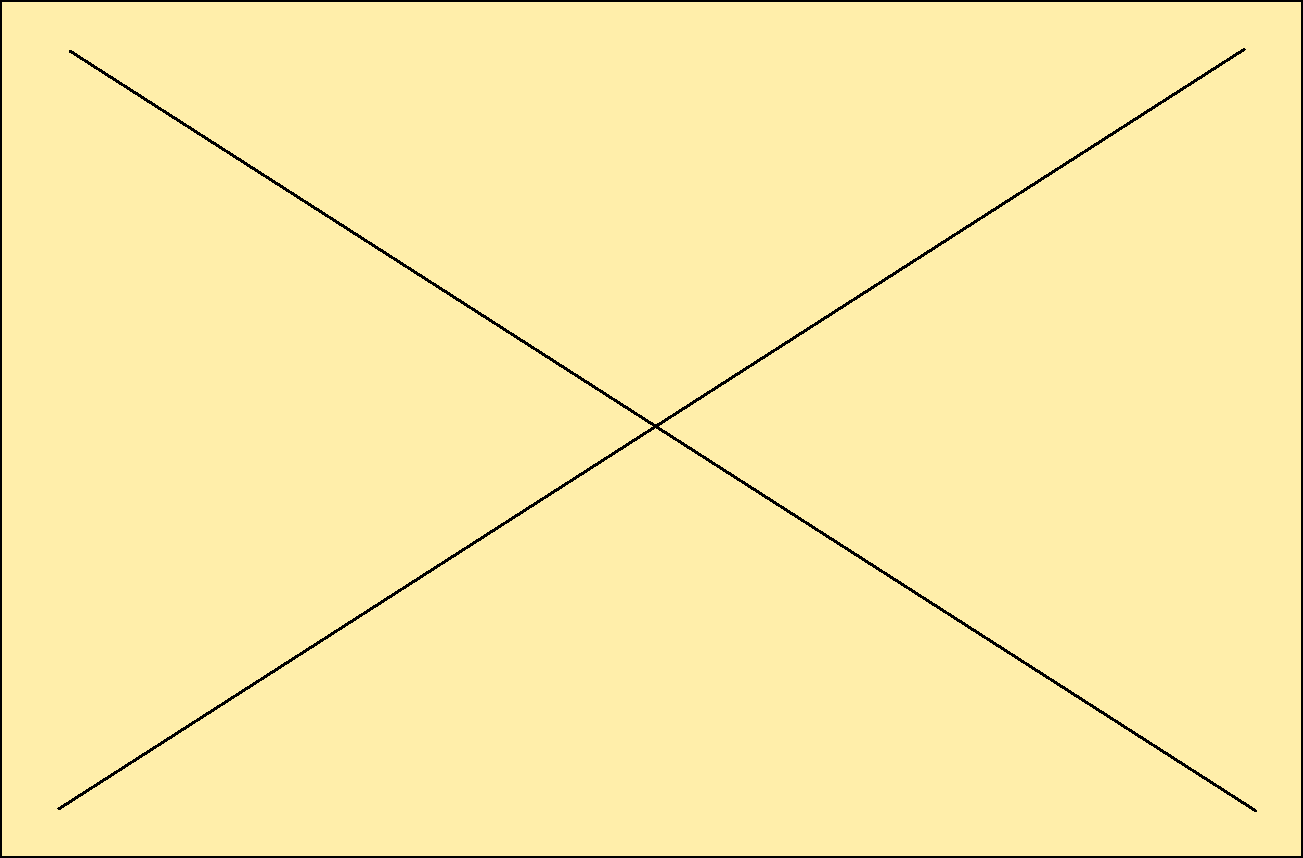
\includegraphics[width=.98\columnwidth]{fig/empty}
%             \caption{With obstacle}
%         \end{subfigure}
%         \hfill
% 		\begin{subfigure}[t]{0.45\hsize}
%         	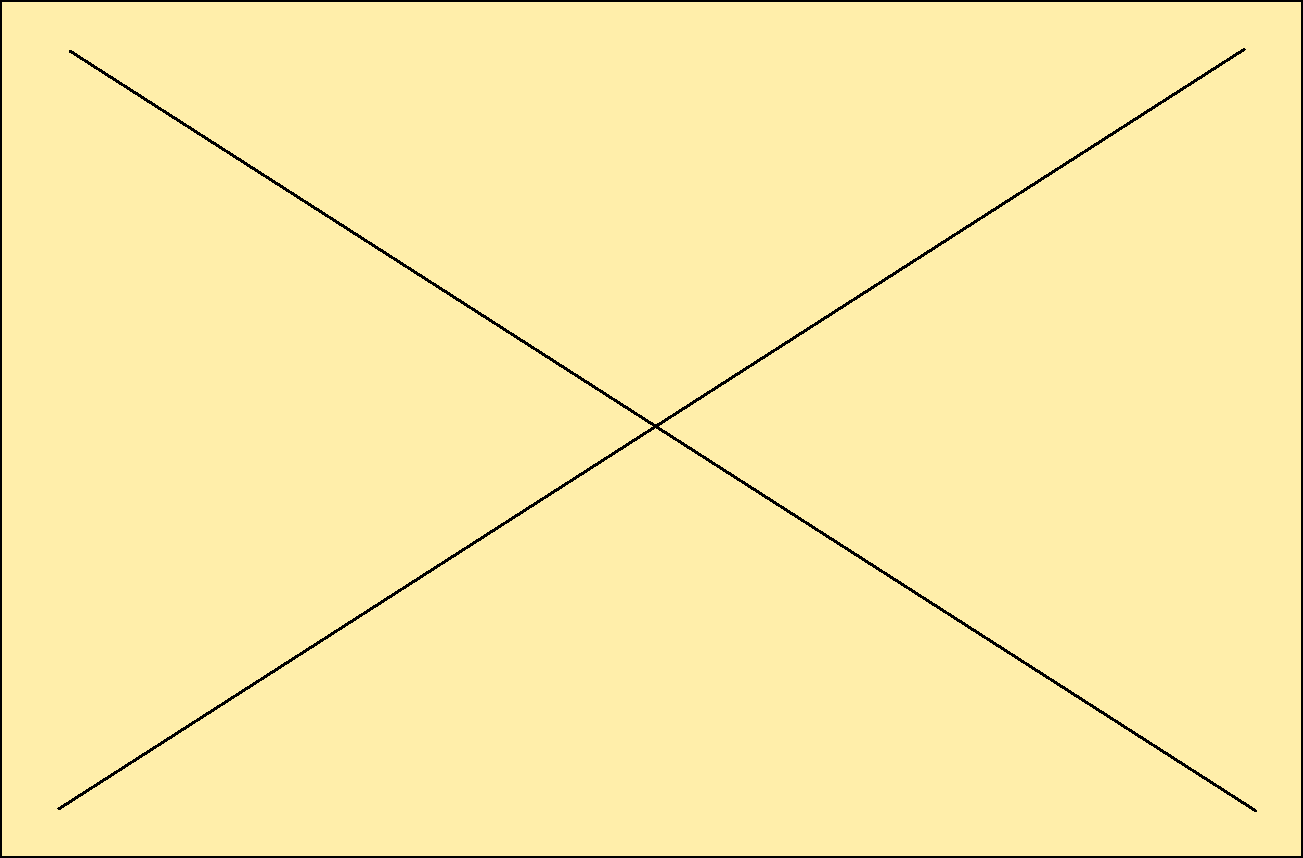
\includegraphics[width=.98\columnwidth]{fig/empty}
%             \caption{Without obstacle}
%         \end{subfigure}
        
% 		\caption{\textbf{\nameref{sec:results:exp2}:} Trajectory of the end effector with and without obstacle.}
% 		\label{fig:slideTraj}
% 	\end{figure}
% 	%


%===============================================================================
 

%%%%%%%%%%%%%%%%%%%%%%%%%%%%%%%%%%%%%%%%%%%%%%%%%%%%%%%%%%%%%%%%%%%%%%%%%%%%%%%%%

\section{Conclusions}
\label{sec:conclusion}

	%\comment{A conclusion section is not required. Although a conclusion may review the main points of the paper, do not replicate the abstract as the conclusion. A conclusion might elaborate on the importance of the work or suggest applications and extensions.}


%The main contribution of this paper is a technique to learn the inverse dynamics model of robots under the effect of multiple and simultaneous contacts exerted on the whole robot structure. 
%In whole-body robot control, estimating contact forces accurately is crucial
%may not only be understood as nuisance that need to be avoided. Making contacts may rather be seen as a desirable feature 
%for balance and stabilization, and to increase the number of potential actions that the robot is able to execute, e.g., reach for distant objects.
%, to stabilize or even . 
Whole-body control strategies that exploit contacts need accurate models of the system dynamics.
%to be stable and precise. 
This is crucial for balance and stabilization, and to increase the number of potential actions that the robot is able to execute, e.g., creating a contact to reach for distant objects.
%
We introduced a data-driven mixture-of-experts approach based on Gaussian processes  for learning inverse dynamics models with contacts. 
% A  was proposed to deal with multiple contacts. %model these non-linear effects. 
We evaluated our model on the \robot{} humanoid robot using tactile sensors and force/torque sensors as model inputs.  
We showed that the model accurately predicts contact forces and outperforms a state-of-the-art analytical approach used to estimate the joint torques in \robot{}. 
The estimation from the learned model does not rely on dynamic parameters, but it is completely data-driven and based on tactile sensors and force/torque sensors. %to determine the amount of external forces.
As a result, our approach does not require a spatially calibrated model of the skin~\cite{DelPrete2011,DelPrete2012}.
% Neither spatially calibrated models of the skin~\cite{DelPrete2011,DelPrete2012} nor preceise knowledge about the contact location were required --- in contrast to the analytical modeling strategy. 
This is a promising feature for robust control strategies that explicitly takes contacts into account. 
%In future, we will incorporate our inverse dynamics models in active control tasks involving multiple contacts in whole-body structure, such as balancing with multiple supports in rigid and compliant environments.

% In future work, we will incorporate our inverse dynamics models in active control tasks using rewards as training signals to overcome the need of labels or ground truth data.

%, which involve multiple simultaneous contacts.
%and as such we could utilize the mixing property of the experts.

% Our solution enables a fast and accurate prediction of the joint torques in situations when the robot is in contact (or not) with an object, detected by a tactile skin.
% The estimation from the learned model does not rely on dynamic parameters, but it is completely data-driven by using tactile sensors and force/torque sensors to determine the amount of external forces.
% As a result, our approach does not requires a spatially calibrated model of the skin~\cite{DelPrete2011,DelPrete2012}.
% With the increasing availability of larger arrays of skin sensors, this kind of data-driven approach greatly reduces the design/engineering complexity.
% %
% %It only introduces an additional sensor measurement $\skinInput$, which provides the information about the contact location and a measure of the applied force on the taxels. 
% Moreover, tactile sensors are cheaper and lighter than joint torque sensors. 
% With our approach, it is possible to apply torque control to robotic manipulators even with contacts at locations other than the end-effector, which makes it possible to control the robot while physically interacting with an evolving environment or humans.

% \todo[inline]{kill this paragraph?\\
% Another advantage of our data-driven approach is that model predictive control needs rapid computation, since it has to compute the entire robot dynamics over a receding time horizon at each control step (as in \cite{naveau2014metapod}, within 1--2~$\mu$s).
% The use of a learned model such as GP potentially allows to reduce the computational time at prediction time and hence to be beneficially used in fast real time applications.}

	%
	\begin{figure}[t]
			\centering
			\includegraphics[width=.94\hsize]{fig/exp5_accuracy_red}
		\caption{\textbf{\nameref{sec:results:exp5}:} Classification accuracy for the heuristic and learned SVM gating networks.
		}
		\label{fig:exp5:accuracy}
        \figspace
	\end{figure}
	% 

%\addtolength{\textheight}{-12cm}   % This command serves to balance the column lengths
                                  % on the last page of the document manually. It shortens
                                  % the textheight of the last page by a suitable amount.
                                  % This command does not take effect until the next page
                                  % so it should come on the page before the last. Make
                                  % sure that you do not shorten the textheight too much.

%%%%%%%%%%%%%%%%%%%%%%%%%%%%%%%%%%%%%%%%%%%%%%%%%%%%%%%%%%%%%%%%%%%%%%%%%%%%%%%%


%%%%%%%%%%%%%%%%%%%%%%%%%%%%%%%%%%%%%%%%%%%%%%%%%%%%%%%%%%%%%%%%%%%%%%%%%%%%%%%%

%\section*{APPENDIX}

%Appendixes should appear before the acknowledgment.


%%%%%%%%%%%%%%%%%%%%%%%%%%%%%%%%%%%%%%%%%%%%%%%%%%%%%%%%%%%%%%%%%%%%%%%%%%%%%%%%

%% Sere: to save some space
%\section*{Acknowledgments}
%
%We thank Vincent Padois and Alain Droniou for their help with \textit{iCubParis02}.
%\medskip
%\noindent
%\textit{Acknowledgments}: 
%\section*{Acknowledgments}
%We thank Vincent Padois and Alain Droniou for their help with \textit{iCubParis02}.

%the iCub facility of the Italian Institute of Technology (IIT) for the technical support provided, and 
%Vincent Padois and Alain Droniou for their help with iCubParis02.
%\fixme{We also thank Vincent \& Alan from UPMC}
 
%
%The research leading to these results has received funding from the European Community's Seventh Framework Programme (FP7/2007--2013) under grant agreements \#270327 (CompLACS) and \#600716 (CoDyCo) and the Department of Computing, Imperial College London.
% The preferred spelling of the word ÒacknowledgmentÓ in America is without an ÒeÓ after the ÒgÓ. Avoid the stilted expression, ÒOne of us (R. B. G.) thanks . . .Ó  Instead, try ÒR. B. G. thanksÓ. Put sponsor acknowledgments in the unnumbered footnote on the first page.


%%%%%%%%%%%%%%%%%%%%%%%%%%%%%%%%%%%%%%%%%%%%%%%%%%%%%%%%%%%%%%%%%%%%%%%%%%%%%%%%

%\clearpage

\bibliographystyle{abbrv}
\bibliography{ICRA2015}



\end{document}